% main.tex - paper 1 (JINST): an algorithm-independent lower limit on
% combinatorial fake tracks. First full draft.
%
% Build:  pdflatex main && bibtex main && pdflatex main && pdflatex main
% The official JINST class (jinst.cls, and JHEP.bst for the references) is
% used if present in this folder; otherwise jinst-fallback.sty stands in.
\IfFileExists{jinst.cls}{\documentclass[a4paper,11pt]{jinst}}
  {\documentclass[a4paper,11pt]{article}\usepackage{jinst-fallback}}
\usepackage{amsmath,amssymb,graphicx,xcolor,booktabs}
\graphicspath{{../example/}{../validation/}{../validation/helix/}}

% ---------------------------------------------------------------- notation
\newcommand{\ndof}{n_\mathrm{dof}}
\newcommand{\Vol}{\mathrm{Vol}}
\newcommand{\dd}{\mathrm{d}}
\newcommand{\todo}[1]{\textcolor{red!70!black}{[#1]}}

\title{An algorithm-independent lower limit on combinatorial fake tracks in high-occupancy tracking detectors}

\author[a,b]{L.~Ristori}
\affiliation[a]{Fermi National Accelerator Laboratory, Batavia, IL 60510, USA}
\affiliation[b]{University of Pisa, Pisa, Italy}
\emailAdd{\todo{to be added}}
% TO DECIDE: author list and affiliations (as they should appear), e-mail address

\abstract{When the density of noise hits in a tracking detector becomes large compared with
its resolution, some random combinations of hits are indistinguishable from real tracks:
they pass the same goodness-of-fit cut that real tracks pass, and no reconstruction
algorithm that keeps the efficiency for real tracks can reject them. We give their expected
number, which is therefore a lower limit on the fake-track rate of any algorithm. It is the
product of the numbers of noise hits on the layers and the probability that one random
combination passes the cut. That probability, which can be as small as $10^{-23}$, follows
from the detector geometry: to leading order it is the number of distinguishable tracks in
the acceptance, times the volume of a $\chi^2$ sphere, divided by the volume of the space of
hit positions, all measured in units of the resolution. We extend the result to tracks
required to have hits on at least $k$ of $N$ layers, check it against direct Monte Carlo
and brute-force counting in small detectors, both for straight lines and for helices in a
solenoidal field, and apply it to a six-layer barrel tower with background levels inspired
by those expected at a muon collider.}

\keywords{Pattern recognition, cluster finding, calibration and fitting methods; Performance of High Energy Physics Detectors; Analysis and statistical methods}

\begin{document}
\flushbottom
\maketitle

% =====================================================================
\section{Introduction}\label{sec:intro}

Track reconstruction in a high-occupancy environment must find the few hits left by charged
particles among many unrelated ones. The problem is familiar at hadron colliders, where
pile-up fills the inner layers~\cite{CMS:2014tracking,ATLAS:2017dense}, and it is extreme at
a muon collider, where the decay products of the circulating muons produce a beam-induced
background of millions of hits per bunch crossing in the tracker~\cite{Accettura:2023,IMCC:2024interim,Casarsa:2024review,Bartosik:2020,Collamati:2021}.
Some of the combinations of background hits happen to line up well enough to be accepted
as tracks. The resulting fake-track rate is normally measured by running a specific
reconstruction algorithm on fully simulated events~\cite{Mankel:2004,Strandlie:2010,Fruhwirth:2021book},
so the number obtained belongs to that algorithm, and possibly to that version of it.

This paper asks a different question: at what hit density does track reconstruction become
impossible for \emph{any} algorithm? The answer exists because a combination of noise hits
that fits a track hypothesis within the resolution carries no information distinguishing it
from a real track. An algorithm that keeps the real tracks that pass a given goodness-of-fit
requirement must also keep these combinations. Their expected number is therefore a lower
limit on the fake rate of every algorithm with that efficiency, and it can be computed from
the detector geometry, the resolution and the hit densities alone.

The expected number is the product of the number of noise hits on each layer and the
probability $P$ that one random combination passes the cut. The difficulty is that $P$ is
tiny: in the example of section~\ref{sec:example} it is $4\times10^{-23}$ for six layers,
far beyond direct simulation. Our earlier work~\cite{Casarsa:2025jinst} (section~8.5)
estimated such probabilities with a Monte Carlo at inflated resolution, scaled back by the
product of the resolution ratios. Here we make that argument exact: $P$ follows a power law
in the cut, $P\simeq K c^{\ndof/2}$, whose exponent is fixed by the number of degrees of
freedom and whose constant $K$ is a geometric quantity, the volume of the set of accepted
tracks in the space of hit positions. It is computed by a low-dimensional integral, with no
Monte Carlo at all.

Related ideas appear in several fields. The probability that $k$ random points are aligned
within a strip of width $w$ scales as $(w/L)^{k-2}$, as found in studies of chance alignments
of random points~\cite{Kendall:1980,Broadbent:1980}; our result contains this law as the
straight-line case. The ``number of false alarms'' of a~contrario detection in image
analysis~\cite{Desolneux:2000} is, like our estimate, an expected number of chance events
that needs no independence assumption. The volume of a tube around a manifold, which gives
our constant $K$, was computed by Hotelling and Weyl~\cite{Hotelling:1939,Weyl:1939} and is
used in statistics for significance tests in nonlinear models~\cite{Johansen:1990,Kuriki:2005}.
Methods that make a rare event common by changing a scale and then extrapolate back are used
in structural reliability~\cite{Bucher:2009,Naess:2009}; here the rescaling is an exact
symmetry and nothing is extrapolated by a fit. In particle physics, the rate of accidental
coincidences between counters~\cite{Leo:1994} and the rate of fake roads in track
triggers~\cite{Ashmanskas:2004svt,Annovi:2013rd13,Ryd:2020trig} are estimated with the same
product-of-occupancies reasoning, but to our knowledge no exact general expression has been
given for combinations accepted by a $\chi^2$ cut.

Section~\ref{sec:defs} defines the problem and states the lower limit, including the common
requirement of hits on at least $k$ of $N$ layers. Section~\ref{sec:method} derives the
probability $P$ for straight tracks. Section~\ref{sec:validation} checks every step against
direct Monte Carlo and brute-force counting. Section~\ref{sec:field} extends the result to
helices in a solenoidal field, and section~\ref{sec:example} applies it to a six-layer
barrel tower. Uncertainties and limitations are discussed in section~\ref{sec:limits}.

% =====================================================================
\section{Definitions and the lower-limit statement}\label{sec:defs}

\paragraph{Detector and noise.} The detector consists of $N$ planar layers. Layer $i$
measures two coordinates of each hit, $u$ and $v$, with Gaussian resolutions $\sigma_{u,i}$
and $\sigma_{v,i}$, over a region of area $A_i$ (in the examples, a square of side $W_i$).
Noise hits are distributed uniformly over each layer, independently of each other, with $n_i$
hits on layer $i$ in the region considered (a fixed number or a Poisson variable of mean
$n_i$; the results are the same).

\paragraph{Acceptance.} A combination of one hit per layer is fitted by least squares to a
track model with $p$ parameters $\theta$; with $m=2N$ measured coordinates the fit has
$\ndof=m-p$ degrees of freedom. The combination is accepted as a track if the fit satisfies
$\chi^2<c$ and the fitted parameters lie in an acceptance region $\Theta$ (for example a
minimum transverse momentum). The cut $c$ is set by the efficiency required for real tracks;
we use a one-sided $3\sigma$ cut, $\Pr(\chi^2_{\ndof}>c)=1.35\times10^{-3}$, which gives
$c=17.80$, $21.74$ and $25.36$ for $\ndof=4$, $6$ and $8$.

\paragraph{The counting identity.} Let $P$ be the probability that one combination of
independent, uniformly distributed hits is accepted. The expected number of accepted noise
combinations is
\begin{equation}
  E = P\prod_{i=1}^{N} n_i ,
  \label{eq:identity}
\end{equation}
by linearity of expectation: $E$ is the sum, over the $\prod_i n_i$ combinations, of the
probability that each is accepted. The identity is exact for the mean even though
combinations that share hits are correlated; correlations affect the variance of the number
of fakes, not its mean.

\paragraph{The lower limit.} A combination of noise hits that passes the cut is, as data, a
valid track: some particle with parameters in $\Theta$ could have produced those hits with
the observed residuals. Consider any algorithm that accepts every combination of hits
compatible with a track in the acceptance, $\chi^2<c$ and $\theta\in\Theta$, so that its
efficiency for real tracks is at least that of the cut. Such an algorithm accepts all the
noise combinations counted by eq.~\eqref{eq:identity}, and $E$ is a lower limit on its number
of fake tracks. An algorithm can of course produce fewer fakes, but only by also losing real
tracks: by tightening $c$ or $\Theta$, which the same formula quantifies, or by rejecting
candidates according to their surroundings, which removes real tracks in the same
surroundings. In this sense, when $E$ approaches one per event the information needed to
reconstruct tracks with the stated efficiency is no longer in the data.

The limit counts only combinations made entirely of noise hits. Combinations in which some
hits belong to a real track and others are noise are also fakes in the usual sense, and
they only add to the number given here.

\subsection{Requiring at least $k$ of $N$ layers}\label{sec:kofn}

Real detectors are inefficient, and track finders usually accept candidates with hits on
at least $k$ of the $N$ layers. Each set $S$ of layers with $|S|\ge k$ then defines its own
fit, with its own number of degrees of freedom and its own cut at the same efficiency for
real tracks: for five of six layers, $\ndof=8$ for the full set and $6$ for each of the six
subsets of five layers. By the same linearity argument, the expected number of accepted
noise combinations is
\begin{equation}
  E(\ge k) = \sum_{|S|\ge k} P_S\prod_{i\in S} n_i ,
  \label{eq:kofn}
\end{equation}
where $P_S$ is the probability for the layers of $S$ alone, computed for their own geometry.
For five of six layers the sum has seven terms. Each term with fewer layers has a larger
probability and one factor $n_i$ less; when the $n_i$ are large but the resolution is good,
as in section~\ref{sec:example}, the five-layer terms dominate by orders of magnitude.

The sum counts combinations, not distinct fake tracks. A six-hit fake usually contains
five-hit subsets that also pass, and two five-hit fakes can share four hits; any algorithm
would merge such candidates. The size of the double counting is set by the \emph{window
occupancy} $\eta$: for an accepted candidate, the expected number of other hits that could
replace one of its hits and still pass, summed over its layers. For layer $i$ of the set,
\begin{equation}
  \eta_i \simeq (n_i-1)\,\frac{\pi\,(c/2)\,\sqrt{(\sigma_{u,i}^2+V_{u,i})(\sigma_{v,i}^2+V_{v,i})}}{A_i},
  \label{eq:eta}
\end{equation}
where $V_{u,i}$, $V_{v,i}$ are the variances of the track position predicted on layer $i$ by
the fit to the other layers, and $c/2$ is the mean $\chi^2$ budget left to the extra hit.
If the number of such neighbours is Poisson with mean $\eta$, the number of distinct fakes is
the number of combinations times $1-\eta/2+O(\eta^2)$. We find that
\begin{equation}
  E_\mathrm{distinct}\simeq e^{-\eta/2}\,E(\ge k)
  \label{eq:distinct}
\end{equation}
describes the straight-line case within a few per cent up to $\eta\approx2$
(section~\ref{sec:validation}). It is exact as $\eta\to0$, which is the regime of interest:
in section~\ref{sec:example}, $\eta\approx0.03$ and the correction is $1.4\%$. We quote
$E_\mathrm{distinct}$ as the lower limit.

% =====================================================================
\section{The probability that one random combination passes}\label{sec:method}

We develop the method for straight tracks (no magnetic field), which contains every
ingredient; section~\ref{sec:field} adds the field.

\paragraph{Whitened coordinates.} Dividing every measured coordinate by its resolution turns
the weighted fit into an unweighted one. A combination of hits becomes a point $x$ in an
$m$-dimensional space, uniformly distributed in a box $B$ whose sides are $W_i/\sigma_{u,i}$
and $W_i/\sigma_{v,i}$, of volume $|B|=\prod_i A_i/(\sigma_{u,i}\sigma_{v,i})$. Each track
$\theta$ produces an ideal point $f(\theta)$, and as $\theta$ runs over the tracks whose hits
lie inside every layer these points form a $p$-dimensional surface $M$, the \emph{track
manifold}. The fit finds the point of $M$ nearest to $x$, and
\begin{equation}
  \chi^2(x) = \min_{\theta}\,\lvert x-f(\theta)\rvert^2
\end{equation}
is the squared distance from $x$ to $M$. Layers of different sizes and resolutions need no
special treatment: in these coordinates every layer is a box, and every acceptance region is
a sphere.

\paragraph{The small-$\chi^2$ law.} The accepted combinations are the points within
distance $\sqrt c$ of $M$: a thin tube around the track manifold. In each of the $\ndof$
directions perpendicular to $M$ the tube is a sphere of radius $\sqrt c$, of volume
$V_{\ndof}\,c^{\ndof/2}$ with $V_d=\pi^{d/2}/\Gamma(d/2+1)$. To leading order its volume is
therefore the area of $M$ times this sphere volume, the result of Hotelling and
Weyl~\cite{Hotelling:1939,Weyl:1939}, and since $x$ is uniform in $B$,
\begin{equation}
  P \simeq K\,c^{\ndof/2},\qquad K = \frac{V_{\ndof}\,\Vol(M)}{|B|},\qquad
  \Vol(M)=\int_{\Theta_B}\sqrt{\det\!\left(J^\mathsf{T}J\right)}\;\dd^p\theta ,
  \label{eq:K}
\end{equation}
where $J=\partial f/\partial\theta$ is the $m\times p$ matrix of derivatives of the whitened
ideal hits with respect to the track parameters, and $\Theta_B$ is the set of parameters in
$\Theta$ whose ideal hits all lie inside the layers (appendix~\ref{app:tube}).

The exponent depends only on the number of degrees of freedom. The constant has a simple
reading: $J^\mathsf{T}J$ is the inverse covariance matrix $C^{-1}$ of the fitted parameters,
so $\Vol(M)=\int \dd^p\theta/\sqrt{\det C}$ is the number of \emph{distinguishable tracks} in
the acceptance, the volume of parameter space counted in units of the parameter errors. The
expected number of fakes is this number of tracks times the probability that, for one of
them, random hits fall inside its $\chi^2$ sphere on every layer. In the example of
section~\ref{sec:example} the six-layer tower contains about $3.5\times10^{14}$
distinguishable tracks.

\paragraph{Corrections.} Equation~\eqref{eq:K} holds when the sphere is small compared with
the layers in whitened units. The leading corrections, from the corners of the acceptance
region and from the curvature of $M$, are of relative order $c$ in units of the whitened
layer size; for a linear track model and a flat boundary the first-order edge effects cancel
(appendix~\ref{app:tube}). We write $P=K c^{\ndof/2}(1+\beta c'+\dots)$, with $c'$ defined
below; in any realistic detector $c'$ is so small that the corrections are negligible.

\paragraph{The straight line.} In each view the track is $u=a+bY$, with $Y$ the depth of the
layer. The Jacobian is constant, $\det(J^\mathsf{T}J)$ is the product over the two views of
$(N\sum_iY_i^2-(\sum_iY_i)^2)/\sigma^4$, and $\Theta_B$ is, in each view, the polygon of
$(a,b)$ for which $|a+bY_i|\le W_i/2$ on every layer. The integral in eq.~\eqref{eq:K}
reduces to the area of that polygon, a one-dimensional integral. The familiar small-argument
form of the $\chi^2$ distribution, $\Pr(\chi^2_{\ndof}<c)\simeq(c/2)^{\ndof/2}/\Gamma(\ndof/2+1)$
for Gaussian residuals~\cite{DLMF}, has the same power for the same geometric reason, with a
different constant because noise hits are uniform rather than Gaussian around a track. For
the alignment of $k$ points in one view, eq.~\eqref{eq:K} reproduces the
$(w/L)^{k-2}$ law of chance alignments~\cite{Kendall:1980,Broadbent:1980}.

\paragraph{Resolution scaling and exact rescaling.} At fixed geometry, $\Vol(M)\propto\sigma^{-p}$
and $|B|\propto\sigma^{-m}$, so at fixed cut
\begin{equation}
  P\propto\sigma^{\ndof},
  \label{eq:sigma}
\end{equation}
and more precisely $P\propto\sigma_u^{\ndof,u}\sigma_v^{\ndof,v}$ when the two views have
different resolutions and $\ndof,u+\ndof,v=\ndof$ degrees of freedom. Equivalently, shrinking
every length of the detector by a factor $\lambda$ at fixed resolution multiplies every
residual by $1/\lambda$ and $\chi^2$ by $1/\lambda^2$, for any track model whose family of
tracks is mapped onto itself (section~\ref{sec:field}). The probability in the real detector
is then exactly that in the shrunken one at a rescaled cut,
\begin{equation}
  P_\mathrm{true}(c)=P_\mathrm{shrunk}(c/\lambda^2).
  \label{eq:rescale}
\end{equation}
We use this identity to test eq.~\eqref{eq:K} by direct Monte Carlo: a detector shrunk until
its smallest layer is two resolutions wide makes accepted combinations common. We call this
the reference detector and $c'=c/\lambda^2$ the cut mapped onto it.

% =====================================================================
\section{Validation}\label{sec:validation}

We test eqs.~\eqref{eq:identity}--\eqref{eq:K} in small projective towers where everything
can be counted: $N=4$ or $6$ layers at depths $Y_i\propto i$, sides $W_i\propto Y_i$,
$\sigma=0.1$~mm in both coordinates. Three tests are made, for straight lines
(figure~\ref{fig:val-line}) and for the exact helix fit of section~\ref{sec:field}
(figure~\ref{fig:val-helix}).

\paragraph{The small-$\chi^2$ law.} For towers of growing size (smaller $c'$) we measure $P$
directly, by fitting random combinations until several hundred pass, and divide it by
$K c'^{\,\ndof/2}$ with $K$ from eq.~\eqref{eq:K}. The ratio tends to one as $c'\to0$. For
straight lines with four layers it is consistent with one within the statistical errors of
$\pm5\%$ for $c'$ from $0.12$ down to $0.004$, where $P=3.7\times10^{-7}$; for six layers,
the points down to $P=3\times10^{-7}$ follow the expected approach from below. For the helix
with four layers the ratio is $0.973$, $0.986$, $1.020$ and $1.013$ ($\pm0.02$--$0.03$) at
$c'=0.070$, $0.031$, $0.017$ and $0.0077$, down to $P=3.5\times10^{-7}$; the six-layer points,
down to $P=4\times10^{-8}$, follow the same trend. At larger $c'$ the ratio falls below one,
as expected from the finite size of the sphere.

\paragraph{The counting identity.} We generate noise-only events and fit \emph{every}
combination: one hit on each of the six layers, and one hit on each layer of every five-layer
subset, each with its own cut, and compare the numbers that pass with
$P_S\prod_{i\in S}n_i$. For straight lines an exact pruning of the combinatorics (a partial
combination already above the cut cannot pass) allows up to 1000 hits per layer and
probabilities $P_S$ down to $10^{-15}$, deep in the small-$\chi^2$ regime; in six
configurations, with 8 to 1000 hits per layer, the ratio of counted to predicted combinations
is between $0.975$ and $1.037$, and $0.990\pm0.008$ combined. For the helix every combination
is fitted by brute force, with 5 to 10 hits per layer; the ratio is $0.97\pm0.03$ over three
configurations, with $P_S$ measured directly in the same geometry.

\paragraph{Distinct fakes.} In the same events, candidates that share four or more hits are
merged and the distinct candidates counted. For straight lines the ratio of distinct fakes to
combinations follows $e^{-\eta/2}$, eq.~\eqref{eq:distinct}, within $1$--$5\%$ for
$0.17\le\eta\le2.2$. For the helix it falls somewhat lower at large occupancy, by a fraction
of about $0.1\,\eta$ ($0.23$ instead of $0.30$ at $\eta=2.4$), and approaches the same
relation as $\eta$ decreases. At the occupancies of interest the difference is negligible.

\paragraph{Why the constant is computed, not fitted.} One could instead fit $K$ to a Monte
Carlo on the reference detector, with a low-order polynomial for the finite-$c'$ corrections.
We find that such fits are biased by a few per cent for straight lines and by up to $10\%$ for
the helix, where the corrections are steeper, and that the result depends on the fitted range
and on the order of the polynomial. Equation~\eqref{eq:K} has no such freedom; its numerical
integration is precise to $10^{-4}$.

\begin{figure}[htbp]
  \centering
  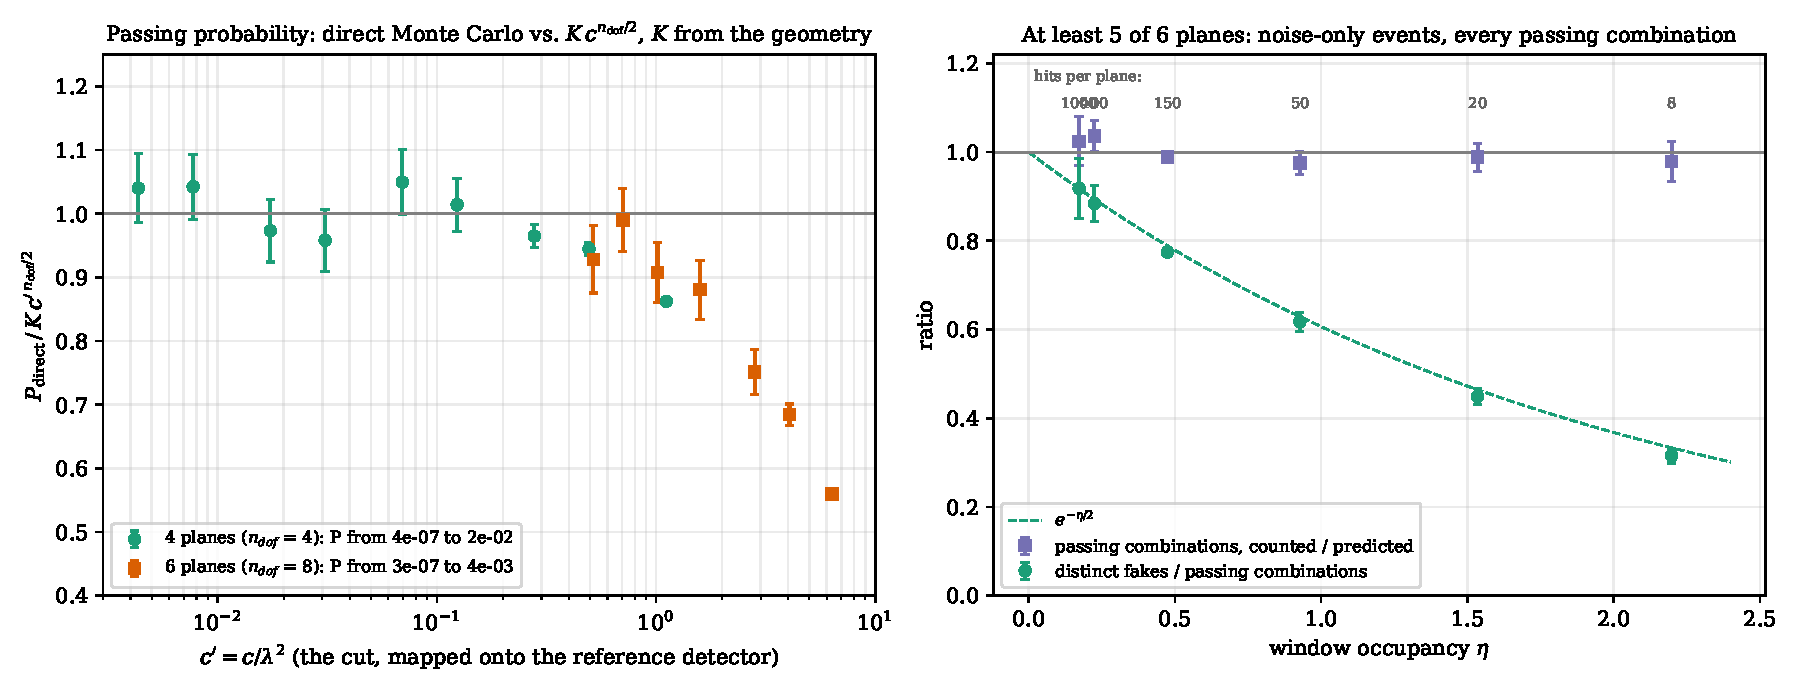
\includegraphics[width=\textwidth]{validation_line}
  \caption{Straight lines. Left: passing probability from direct Monte Carlo divided by
  $K c'^{\,\ndof/2}$, with $K$ from eq.~\eqref{eq:K}, against the cut mapped onto the reference
  detector, for towers of four and six layers. Right: noise-only events in which every
  combination is fitted, for at least five of six layers; ratio of counted to predicted
  passing combinations, and ratio of distinct fakes (candidates sharing four or more hits
  merged) to combinations, against the window occupancy $\eta$. The numbers of hits per layer
  are given above the points.}
  \label{fig:val-line}
\end{figure}

\begin{figure}[htbp]
  \centering
  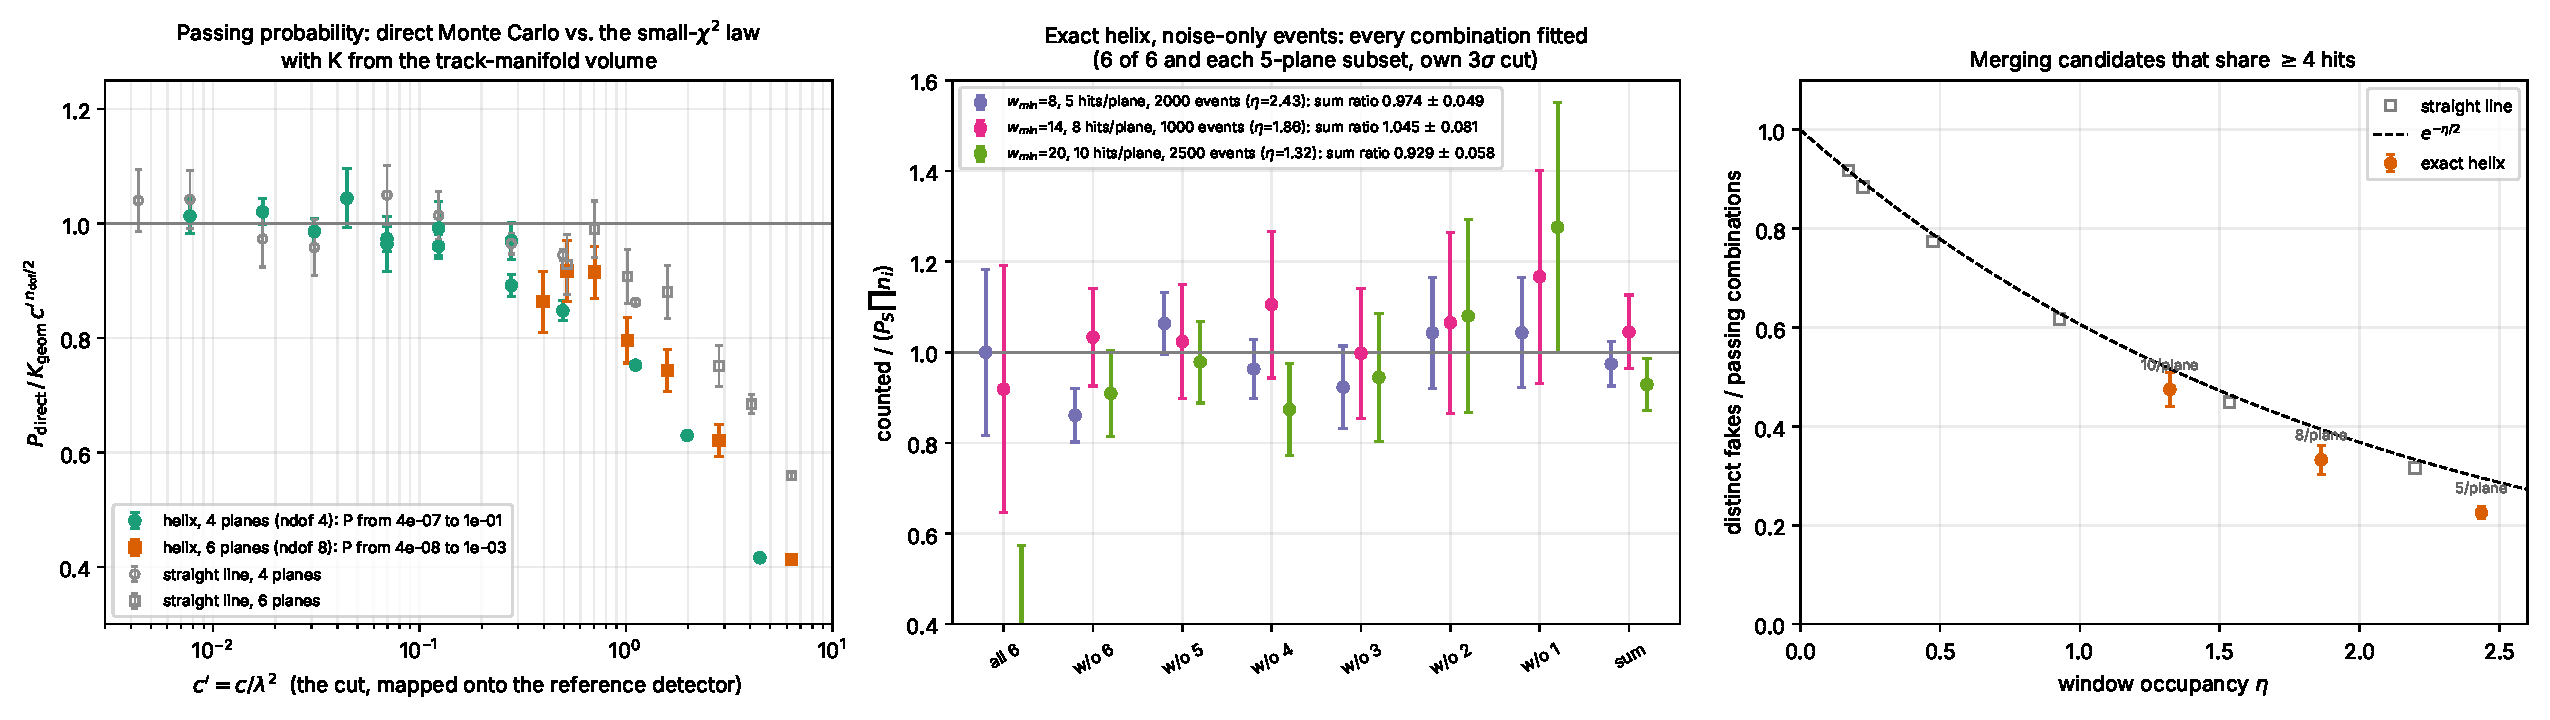
\includegraphics[width=\textwidth]{validation_helix}
  \caption{Exact helix fit. Left: as figure~\ref{fig:val-line}, for four and six layers, with
  the straight-line points in grey. Middle: counted over predicted passing combinations for
  six of six layers and for each five-layer subset, in three configurations. Right: distinct
  fakes over passing combinations against $\eta$, with the straight-line points for
  comparison.}
  \label{fig:val-helix}
\end{figure}

% =====================================================================
\section{Tracks in a solenoidal field}\label{sec:field}

\paragraph{Track model.} In a uniform axial field we consider tracks from the beam line, with
the layers at depths $Y_i$ measuring the bending coordinate $X$ and the coordinate $Z$ along
the field. In the bending plane the track is an exact circle through the origin, with
initial slope $b$ and signed curvature $\kappa$:
\begin{equation}
  X(Y;b,\kappa)=\frac{1}{\kappa\sqrt{1+b^2}}-\operatorname{sgn}(\kappa)\sqrt{\kappa^{-2}-\left(Y+\frac{b}{\kappa\sqrt{1+b^2}}\right)^{2}} .
\end{equation}
Along the field the track is a straight line in the path length; we write
$Z=p+q\,r$, with $r=\sqrt{X^2+Y^2}$ the transverse distance from the beam line, which differs
from the path length by a relative amount $(\kappa r)^2/24$, at most $2\times10^{-3}$ in our
example; its effect on $K$ is smaller still. The fit has $p=4$ parameters and $\ndof=2N-4$.
The acceptance requires $|\kappa|\le\kappa_\mathrm{max}$, which corresponds to a minimum
transverse momentum $p_T>0.3\,B/\kappa_\mathrm{max}$ (in GeV/$c$, tesla and metres).

\paragraph{The fit.} The bending view has no closed-form solution. We minimize it with the
Levenberg--Marquardt method~\cite{Levenberg:1944,Marquardt:1963}, started from several
values of the curvature spread over the acceptance, and keep the lowest $\chi^2$; the depth
view, given the bending fit, is linear. A single starting point would occasionally converge
to a local minimum, overestimate $\chi^2$ and underestimate the number of fakes. The direct
Monte Carlo of section~\ref{sec:validation} uses the same fit: its agreement with the
geometric $K$, which assumes the global minimum, shows that the minimum is found. Algebraic
circle fits~\cite{Karimaki:1991} could be used to seed the minimization.

\paragraph{The constant $K$.} The track manifold is now curved, but eq.~\eqref{eq:K} still
holds to leading order. The Jacobian has a block structure: the bending coordinates depend
only on $(b,\kappa)$, and the depth coordinates on $(p,q)$ and, through $r$, on $(b,\kappa)$.
The volume element factorizes into the bending-view determinant and the depth-view
determinant $(N\sum_i r_i^2-(\sum_i r_i)^2)/\sigma^4$ (appendix~\ref{app:tube}), and
\begin{equation}
  \Vol(M)=\int\!\dd b\,\dd\kappa\;\sqrt{\det\!\left(J_X^\mathsf{T}J_X\right)}\;
  \frac{\sqrt{N\sum_i r_i^2-(\sum_i r_i)^2}}{\sigma^2}\;\mathcal{A}(b,\kappa),
\end{equation}
where $\mathcal{A}(b,\kappa)$ is the area of the polygon of $(p,q)$ whose hits lie inside every
layer. The remaining two-dimensional integral is computed on a grid; $400\times400$ points
give $K$ to $10^{-4}$ in about a minute.

\paragraph{Rescaling and the curvature acceptance.} Shrinking every length by $\lambda$ maps a
circle of curvature $\kappa$ onto one of curvature $\lambda\kappa$; with
$\kappa_\mathrm{max}\to\lambda\kappa_\mathrm{max}$ the family of accepted tracks is mapped
onto itself and eq.~\eqref{eq:rescale} remains exact. We checked numerically that $\chi^2$
scales as $\lambda^{-2}$ and the fitted curvature as $\lambda$ to $10^{-4}$. Since the
bending-view volume element varies slowly with $\kappa$ at small curvature, $K$ is nearly
proportional to $\kappa_\mathrm{max}$, that is to $1/p_{T,\min}$.

% =====================================================================
\section{Worked example: a six-layer barrel tower}\label{sec:example}

\paragraph{Geometry and hit densities.} We consider a barrel tower whose radii and hit
densities are inspired by the tracker designs and background studies for a 10~TeV muon
collider~\cite{Andreetto:2026music,Bell:2025maia,Bartosik:2020,Collamati:2021}, rounded to two
significant figures (table~\ref{tab:example}). The tower is projective, with layers at
$Y=160$, $350$, $550$, $820$, $1200$ and $1500$~mm and an outermost layer of $1~\mathrm{m}^2$;
the hit densities are those expected after background-suppression cuts on hit time and
direction. We take $\sigma=100~\mu$m in both coordinates, a time resolution of $100$~ps for
the timing cut that produces these densities, $B=5$~T and $p_T>10$~GeV/$c$. These are
conventional, present-day assumptions; the detector of a future muon collider may do better.

\begin{table}[htbp]
  \centering
  \caption{The six-layer tower of the worked example.}
  \label{tab:example}
  \begin{tabular}{crrrr}
    \toprule
    layer & $Y$ (mm) & $W$ (mm) & density (hits/mm$^2$) & hits per layer $n_i$ \\
    \midrule
    1 & 160  & 107  & 0.039   & 444 \\
    2 & 350  & 233  & 0.011   & 599 \\
    3 & 550  & 367  & 0.0036  & 484 \\
    4 & 820  & 547  & 0.0013  & 388 \\
    5 & 1200 & 800  & 0.00083 & 531 \\
    6 & 1500 & 1000 & 0.00053 & 530 \\
    \bottomrule
  \end{tabular}
\end{table}

\paragraph{Results.} Table~\ref{tab:example-results} gives, for each set of layers, the
probability that one random combination passes and the expected number of accepted
combinations per tower and event. With six of six layers, $P=3.7\times10^{-23}$ and
$E=5.2\times10^{-7}$. Each five-layer subset has a probability larger by about six orders of
magnitude and one factor of about 500 hits less, so its term is larger by two to three orders
of magnitude; the sum, for at least five of six layers, is $E=3.8\times10^{-3}$. The window
occupancy is $\eta=0.010$--$0.031$, so the number of distinct fakes is $0.986$ times the sum,
$3.7\times10^{-3}$ per tower and event. At these values of the cut, $c'\approx10^{-4}$ on the
reference detector, and the finite-$c$ corrections are of order $10^{-5}$.

\begin{table}[htbp]
  \centering
  \caption{Fake probability $P_S$, expected number of accepted combinations $E_S$ per tower and
  event, and window occupancy $\eta$ for each set of layers of the worked example
  ($\sigma=100~\mu$m, $p_T>10$~GeV/$c$, $B=5$~T).}
  \label{tab:example-results}
  \begin{tabular}{lcccc}
    \toprule
    layers & $\ndof$ & $P_S$ & $E_S$ & $\eta$ \\
    \midrule
    all six           & 8 & $3.7\times10^{-23}$ & $5.2\times10^{-7}$ & 0.031 \\
    without layer 6   & 6 & $3.6\times10^{-17}$ & $9.5\times10^{-4}$ & 0.030 \\
    without layer 5   & 6 & $5.1\times10^{-17}$ & $1.4\times10^{-3}$ & 0.029 \\
    without layer 4   & 6 & $2.6\times10^{-17}$ & $9.3\times10^{-4}$ & 0.027 \\
    without layer 3   & 6 & $1.2\times10^{-17}$ & $3.4\times10^{-4}$ & 0.028 \\
    without layer 2   & 6 & $4.7\times10^{-18}$ & $1.1\times10^{-4}$ & 0.026 \\
    without layer 1   & 6 & $2.5\times10^{-18}$ & $7.8\times10^{-5}$ & 0.010 \\
    \midrule
    at least 5 of 6   &   &                     & $3.8\times10^{-3}$ &       \\
    \bottomrule
  \end{tabular}
\end{table}

\paragraph{Headroom.} Figure~\ref{fig:example} shows how the limit grows with the hit density
and with the resolution. Multiplying all densities by a common factor $\mu$ multiplies each
term by $\mu^{|S|}$: the sum, dominated by the five-layer terms, grows as $\mu^5$ and reaches
one fake per tower at $\mu=3.0$. At fixed densities, degrading the position resolution by a
factor $f$ multiplies the five-layer terms by $f^6$ and the six-layer term by $f^8$; one fake
is reached at $\sigma=250~\mu$m. In a real detector the cuts that produce the densities would
also depend on the resolution, so this second curve isolates the effect of the fake
probability alone.

\begin{figure}[htbp]
  \centering
  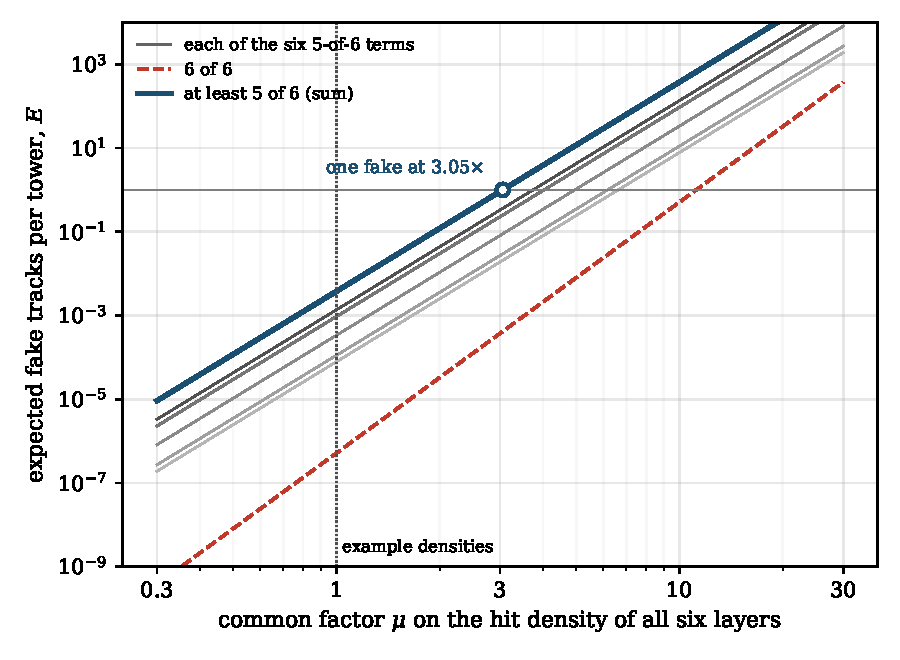
\includegraphics[width=0.49\textwidth]{example_density}\hfill
  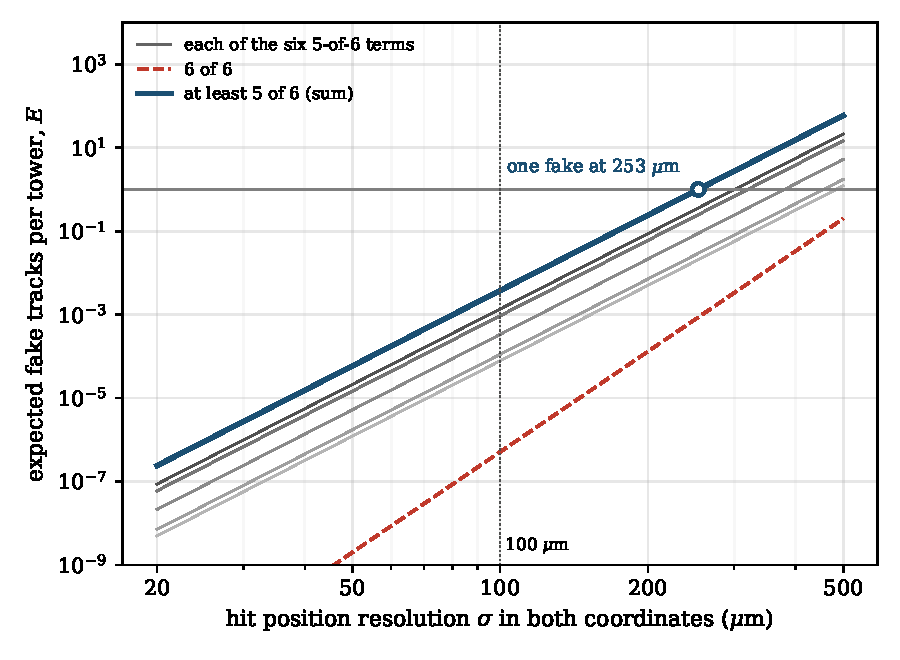
\includegraphics[width=0.49\textwidth]{example_resolution}
  \caption{Expected fake tracks per tower in the worked example. Left: against a common factor
  on the hit densities of all six layers. Right: against the hit position resolution (the
  same in both coordinates), at fixed densities. Thick line: at least five of six layers;
  thin lines: the six five-layer terms (two of them nearly coincide); dashed: six of six.}
  \label{fig:example}
\end{figure}

% =====================================================================
\section{Uncertainties and limitations}\label{sec:limits}

\paragraph{Numerical.} The integral of eq.~\eqref{eq:K} is computed to $10^{-4}$, and the
finite-$c$ corrections in the example are of order $10^{-5}$. The fit finds the global minimum
(section~\ref{sec:field}). The validation of section~\ref{sec:validation} tests the complete
chain at the level of a few per cent, limited by Monte Carlo statistics.

\paragraph{Assumptions.} The resolution is taken as Gaussian without tails, and multiple
scattering is neglected, which is adequate for the high-$p_T$ tracks of the example. The
tower is an idealized projective geometry with flat layers, and the noise is uniform within
each layer. A non-uniform density enters eq.~\eqref{eq:K} as a weight in the same integral;
with the mean density, the result holds when the density varies slowly on the scale of the
fit windows. The model of the path length along the field (section~\ref{sec:field}) affects $K$
by less than $10^{-3}$.

\paragraph{What the limit does not include.} Combinations mixing hits of real tracks with
noise, correlated noise (clusters of hits from one particle, low-momentum particles curling in
the field) and inefficiency of real tracks all add fakes or remove real tracks; none can
lower the limit.

% =====================================================================
\section{Conclusions}\label{sec:conclusions}

The expected number of combinations of noise hits that pass the goodness-of-fit cut of a
track fit is a lower limit on the fake-track rate of any reconstruction algorithm that keeps
the efficiency for real tracks given by that cut. It is the product of the numbers of noise
hits on the layers and a probability that follows from geometry: the number of
distinguishable tracks in the acceptance times the volume of the $\chi^2$ sphere, divided by
the volume of the space of hit positions, everything in units of the resolution. The
probability is computed by a low-dimensional integral, with no Monte Carlo, for straight
lines and for helices in a solenoidal field, and its validity has been checked by direct
Monte Carlo and by counting every combination in small detectors.

The limit grows as the $k$-th power of a common hit density for tracks with at least $k$ of
$N$ layers, and as the $\ndof$-th power of the resolution. When hits may be missing, the sets
with the fewest layers dominate, by orders of magnitude. For a six-layer barrel tower with
background levels inspired by those expected at a muon collider, a resolution of $100~\mu$m and
at least five of six layers, the limit is $4\times10^{-3}$ fake tracks per tower and event:
reconstruction is possible, but a three-fold increase in hit density or a 2.5-fold degradation
of the resolution would make it impossible for any algorithm. The method gives this kind of
statement for any detector from its geometry, resolution and expected occupancy alone, and can
be used early in the design of a tracker to set requirements on resolution and background
rejection.

% =====================================================================
\appendix
\section{Notation}\label{app:notation}

\begin{tabular}{ll}
  $N$, $k$ & number of layers; minimum number of layers required \\
  $S$ & a set of layers; $|S|$ its size \\
  $Y_i$, $W_i$, $A_i$ & depth, side and area of layer $i$ \\
  $\sigma_{u,i}$, $\sigma_{v,i}$ & resolutions of the two measured coordinates \\
  $n_i$, $\rho_i$ & noise hits on layer $i$; density $n_i/A_i$ \\
  $m$, $p$, $\ndof$ & measured coordinates ($2N$), track parameters, degrees of freedom \\
  $c$ & cut on $\chi^2$ \\
  $\Theta$, $\Theta_B$ & acceptance; parameters whose hits lie inside every layer \\
  $f(\theta)$, $J$ & whitened ideal hits of track $\theta$; $J=\partial f/\partial\theta$ \\
  $M$, $\Vol(M)$ & track manifold; its $p$-dimensional volume \\
  $B$, $|B|$ & whitened box of hit positions; its volume \\
  $V_d$ & volume of the unit sphere in $d$ dimensions \\
  $P$, $K$ & probability that one combination passes; $P\simeq Kc^{\ndof/2}$ \\
  $E$, $E(\ge k)$ & expected number of accepted combinations \\
  $\eta$ & window occupancy \\
  $\lambda$, $c'$ & shrink factor; cut mapped onto the reference detector \\
  $b$, $\kappa$, $p$, $q$ & helix parameters: slope and curvature; depth-view intercept and slope \\
\end{tabular}

\section{The track-manifold volume}\label{app:tube}

\paragraph{The tube.} Near the track manifold, write each point of the hit space as
$x=f(\theta)+\sum_{j=1}^{\ndof}t_j\,n_j(\theta)$, with $n_j(\theta)$ an orthonormal basis of the
directions perpendicular to $M$ at $f(\theta)$. For a point close to $M$, $\chi^2(x)=|t|^2$,
and the fitted parameters are $\theta$. The volume element is
$\dd^m x=\sqrt{\det(J^\mathsf{T}J)}\,(1+O(|t|/R))\,\dd^p\theta\,\dd^{\ndof}t$, with $R$ the
radius of curvature of $M$. Integrating $t$ over the sphere $|t|<\sqrt c$ and $\theta$ over
$\Theta_B$ gives eq.~\eqref{eq:K}. For a linear model, $R=\infty$ and the expansion is exact
away from the boundary of $B$.

\paragraph{The boundary.} Near a face of the box $B$, part of the sphere around a point of $M$
inside $B$ lies outside, and part of the sphere around a point just outside lies inside. For
a linear model and a flat face, a displacement $t$ shifts the boundary of the accepted
parameters linearly in $t$, and the average over the sphere vanishes: the two effects cancel
to first order. The leading corrections come from the corners of $B$ and from the curvature
of $M$, and are of relative order $c$ in units of the whitened layer size.

\paragraph{The depth view of the helix.} The depth fit uses the measured bending coordinate in
$r_i=\sqrt{X_i^2+Y_i^2}$. To first order in the residuals, a residual $\delta X_i$ shifts the
depth residual by $q\,(X_i/r_i)\,\delta X_i$. This is a shear of the hit space, of unit
Jacobian, that leaves the volume unchanged: in sheared coordinates the bending and depth
residuals are independent, and the volume element is the product of the bending-view
determinant and the depth-view determinant evaluated at the ideal $r_i$.

\section{Constants}\label{app:constants}

\begin{table}[htbp]
  \centering
  \caption{The constant $K$ of eq.~\eqref{eq:K} for the configurations of this paper. Validation
  towers: layers at $Y_i\propto i$, $W_i\propto Y_i$, $\sigma=0.1$~mm, smallest layer $2\sigma$
  wide (straight line: $Y_i=100\,i$~mm; helix: $W_i=0.673\,Y_i$, $\kappa_\mathrm{max}Y_N=0.2$).
  Layers are numbered from the inside out.}
  \label{tab:K}
  \small
  \begin{tabular}{llcl}
    \toprule
    configuration & layers & $\ndof$ & $K$ \\
    \midrule
    straight line, 4 layers & all & 4 & $1.904\times10^{-2}$ \\
    straight line, 6 layers & all & 8 & $4.624\times10^{-6}$ \\
                            & w/o 6, 5, 4, 3, 2, 1 & 6 & $4.381$, $4.149$, $3.086$, $1.736$, $0.664$, $0.701\times10^{-4}$ \\
    helix, 4 layers         & all & 4 & $5.833\times10^{-3}$ \\
    helix, 6 layers         & all & 8 & $2.043\times10^{-6}$ \\
                            & w/o 6, 5, 4, 3, 2, 1 & 6 & $1.385$, $1.855$, $1.297$, $0.698$, $0.297$, $0.171\times10^{-4}$ \\
    worked example          & all & 8 & $8.856\times10^{-29}$ \\
                            & w/o 6, 5, 4, 3, 2, 1 & 6 & $3.486$, $5.010$, $2.500$, $1.124$, $0.462$, $0.240\times10^{-21}$ \\
    \bottomrule
  \end{tabular}
\end{table}

\section{Code and data availability}\label{app:code}

The code that computes $K$ for any set of layers, the validation Monte Carlo and the worked
example, and the scripts that produce every number and figure of this paper, are available in
a public repository~\cite{code}. \todo{Archive the version used (e.g.\ Zenodo) and give its
DOI.}

% =====================================================================
\acknowledgments
\todo{To be written.}

\paragraph{Use of AI tools.}
\todo{Draft, to be checked against the IOP Publishing policy at submission.} The author used
Claude (Anthropic; model Claude Opus~5.5) as an assistant to write and test the simulation and
analysis code, to run the Monte Carlo validations, to search the literature, and to draft parts
of the text and figures. All results were checked by the author: the code is
public~\cite{code}, every number in the paper is reproduced by its scripts, and the method was
validated independently as described in section~\ref{sec:validation}. The author takes full
responsibility for the content of this paper.

% =====================================================================
\IfFileExists{JHEP.bst}{\bibliographystyle{JHEP}}{\bibliographystyle{unsrt}}
\bibliography{refs}

\end{document}
